\documentclass[conference]{IEEEtran}

%%%%%%%%%%%%%%%%%%%%%%%%%%%%%%%%%%%%%%%%%%%%%%%%%%%%%%%%%%%%%%%%%%%%%%%%%%%%%%%%%%%%%%%%%%%%%%%%%%%%%%%%%%
\usepackage{amsmath,bm}
\usepackage{graphicx}

\def\MLine#1{\par\hspace*{-\leftmargin}\parbox{\textwidth}{\[#1\]}}
\graphicspath{ {./Images/} }
%%%%%%%%%%%%%%%%%%%%%%%%%%%%%%%%%%%%%%%%%%%%%%%%%%%%%%%%%%%%%%%%%%%%%%%%%%%%%%%%%%%%%%%%%%%%%%%%%%%%%%%%%%

%%%%%%%%%%%%%%%%%%%%%%%%%%%%%%%%%%%%%%%%%%%%%%%%%%%%%%%%%%%%%%%%%%%%%%%%%%%%%%%%%%%%%%%%%%%%%%%%%%%%%%%%%%
\begin{document}
%%%%%%%%%%%%%%%%%%%%%%%%%%%%%%%%%%%%%%%%%%%%%%%%%%%%%%%%%%%%%%%%%%%%%%%%%%%%%%%%%%%%%%%%%%%%%%%%%%%%%%%%%%
\title{Software systems}
\author{Xin Wang}
%%%%%%%%%%%%%%%%%%%%%%%%%%%%%%%%%%%%%%%%%%%%%%%%%%%%%%%%%%%%%%%%%%%%%%%%%%%%%%%%%%%%%%%%%%%%%%%%%%%%%%%%%%
\maketitle
%%%%%%%%%%%%%%%%%%%%%%%%%%%%%%%%%%%%%%%%%%%%%%%%%%%%%%%%%%%%%%%%%%%%%%%%%%%%%%%%%%%%%%%%%%%%%%%%%%%%%%%%%%
\section{\textbf{Overview}}
%%%%%%%%%%%%%%%%%%%%%%%%%%%%%%%%%%%%%%%%%%%%%%%%%%%%%%%%%%%%%%%%%%%%%%%%%%%%%%%%%%%%%%%%%%%%%%%%%%%%%%%%%%
\subsection{Analysing software systems}

\begin{itemize}
    \item Aspects to consider:
    \begin{itemize}
        \item System high-level functions
        \item System nodes
        \item Types of data managed and processed
        \item Data movement within the system
    \end{itemize}

    \item Usually expressed with pictures
\end{itemize}

%%%%%%%%%%%%%%%%%%%%%%%%%%%%%%%%%%%%%%%%%%%%%%%%%%%%%%%%%%%%%%%%%%%%%%%%%%%%%%%%%%%%%%%%%%%%%%%%%%%%%%%%%%
\subsection{Modelling data (Database)}

\begin{itemize}
    \item Data is always stored, transformed and analysed
    \item \textbf{Abstract Data Model} used to understand process
    \item \textbf{Database theory} creates the Abstract Data Model
    \item Database theory considers:
    \begin{itemize}
        \item Important entities in Database
        \item \textbf{Attributes} of these entities
        \item \textbf{Relationships} between these entities
    \end{itemize}
    \item \textbf{Entity modelling} formally expresses database theory
    \item \textbf{Database systems} implements the Abstract Data Model
\end{itemize}

%%%%%%%%%%%%%%%%%%%%%%%%%%%%%%%%%%%%%%%%%%%%%%%%%%%%%%%%%%%%%%%%%%%%%%%%%%%%%%%%%%%%%%%%%%%%%%%%%%%%%%%%%%
\subsection{Moving data (Network)}

\begin{itemize}
    \item Process of data moving between nodes
    \item \textbf{Network models} defines the type of network structure
    \item \textbf{Network protocol} and \textbf{API} implements the model
\end{itemize}

%%%%%%%%%%%%%%%%%%%%%%%%%%%%%%%%%%%%%%%%%%%%%%%%%%%%%%%%%%%%%%%%%%%%%%%%%%%%%%%%%%%%%%%%%%%%%%%%%%%%%%%%%%
\section{\textbf{Entity Relation Modelling}}
%%%%%%%%%%%%%%%%%%%%%%%%%%%%%%%%%%%%%%%%%%%%%%%%%%%%%%%%%%%%%%%%%%%%%%%%%%%%%%%%%%%%%%%%%%%%%%%%%%%%%%%%%%
\begin{itemize}
    \item Creates \textbf{Entity Relationship Diagram}
    \item Establishing \textbf{relationships} in a given system:
    \begin{itemize}
        \item \textbf{Entities}: Aspects within a given system
        \item \textbf{Relationships}: How entities are related
        \item \textbf{Attributes}: Properties of an entity or relationship
    \end{itemize}
    \item Captures constraints and requirements on data 
    \item Used as a guide to \textit{implement} relations
\end{itemize}
\begin{figure} [h!]
    \centering
    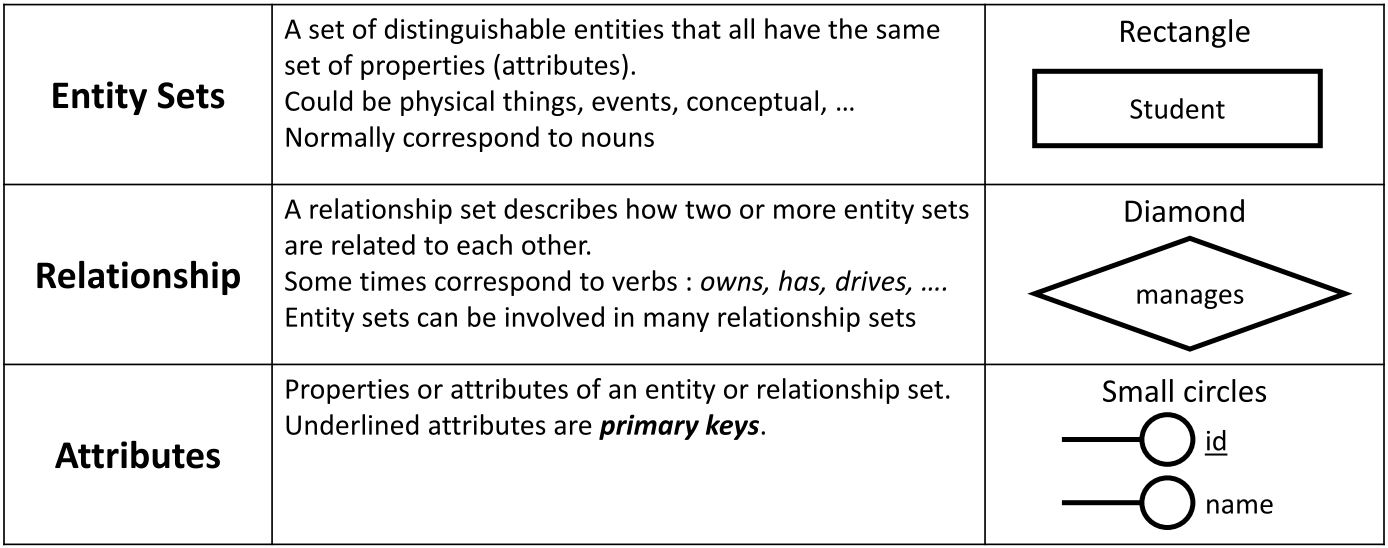
\includegraphics[scale=0.3]{ERM.JPG}
\end{figure}

%%%%%%%%%%%%%%%%%%%%%%%%%%%%%%%%%%%%%%%%%%%%%%%%%%%%%%%%%%%%%%%%%%%%%%%%%%%%%%%%%%%%%%%%%%%%%%%%%%%%%%%%%%
\subsection{Primary keys}

\begin{itemize}
    \item An attribute that \textbf{uniquely identifies} an entity
    \item Properties:
    \begin{itemize}
        \item There will never be two entities with the same key 
        \item Can contain \textbf{multiple} attributes if needed
        \item Shown on ERD as \underline{underlined attributes}
    \end{itemize}
    \item Two types of primary keys:
    \begin{itemize}
        \item \textbf{Natural keys}: Attributes from application data 
        \item \textbf{Surrogate keys}: \textit{Invented} attributes 
    \end{itemize}
\end{itemize}
\begin{figure} [h!]
    \centering
    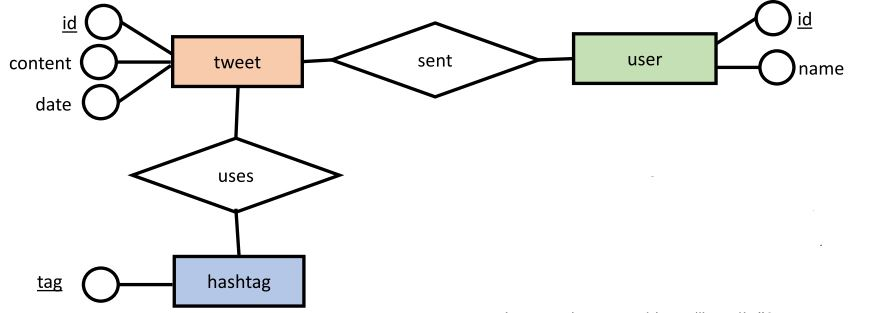
\includegraphics[scale=0.4]{Ex2.JPG}
\end{figure}

%%%%%%%%%%%%%%%%%%%%%%%%%%%%%%%%%%%%%%%%%%%%%%%%%%%%%%%%%%%%%%%%%%%%%%%%%%%%%%%%%%%%%%%%%%%%%%%%%%%%%%%%%%
\subsection{Complex attributes}

\begin{itemize}
    \item \textbf{Computed attributes}: Calculated from other attributes
    \begin{figure} [h!]
        \centering
        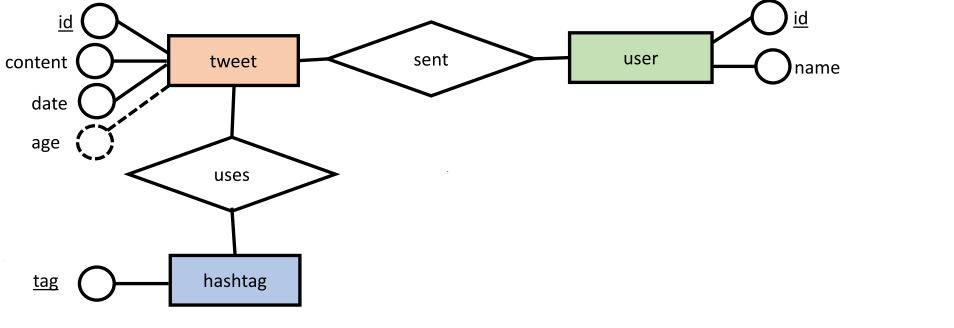
\includegraphics[scale=0.4]{Ex3.JPG}
    \end{figure}
    \item \textbf{Multi-valued attributes}: Sets or lists of multiple values
    \begin{figure} [h!]
        \centering
        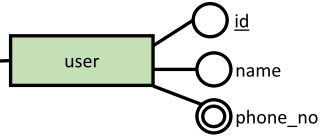
\includegraphics[scale=0.4]{Ex4.JPG}
    \end{figure}
    \item \textbf{Composite attributes}: Properties that has sub-attributes
    \begin{figure} [h!]
        \centering
        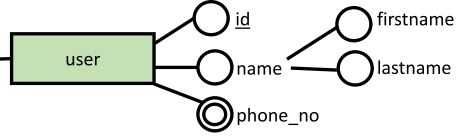
\includegraphics[scale=0.4]{Ex5.JPG}
    \end{figure}
\end{itemize}

\pagebreak

%%%%%%%%%%%%%%%%%%%%%%%%%%%%%%%%%%%%%%%%%%%%%%%%%%%%%%%%%%%%%%%%%%%%%%%%%%%%%%%%%%%%%%%%%%%%%%%%%%%%%%%%%%
\section{\textbf{Relationships: Sets of relations}}

\begin{itemize}
    \item Entity sets contain distinct entities 
    \item \textbf{Relationships} contain sets of relations 
    \item Each \textbf{relation} is a \textit{pair of links} to an entity in the two entity sets
\end{itemize}
\begin{figure} [h!]
    \centering
    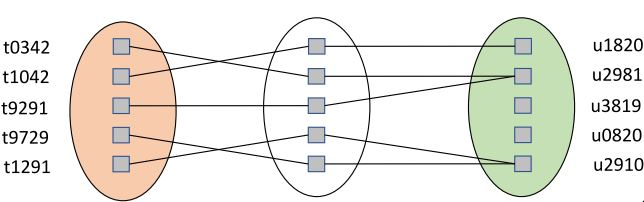
\includegraphics[scale=0.4]{Ex6.JPG}
\end{figure}

%%%%%%%%%%%%%%%%%%%%%%%%%%%%%%%%%%%%%%%%%%%%%%%%%%%%%%%%%%%%%%%%%%%%%%%%%%%%%%%%%%%%%%%%%%%%%%%%%%%%%%%%%%
\subsection{Relation constraints}

\begin{itemize}
    \item \textbf{Cardinality constraint}: Number of times entity appears 
    \begin{itemize}
        \item One-to-one
        \item One-to-many
        \begin{figure} [h!]
            \centering
            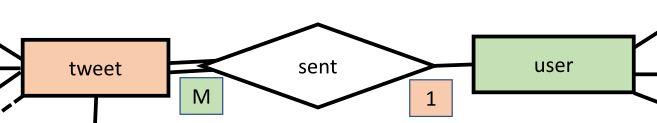
\includegraphics[scale=0.4]{Ex8.JPG}
        \end{figure}
        \item Many-to-many
        \begin{figure} [h!]
            \centering
            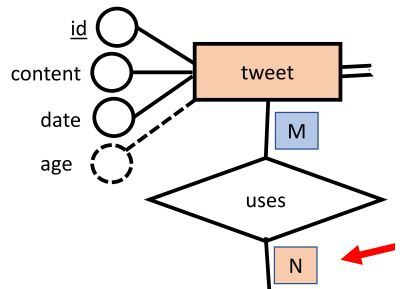
\includegraphics[scale=0.4]{Ex9.JPG}
        \end{figure}
    \end{itemize}
    \item \textbf{Total participation}: Entities \textbf{must} appear in relationships
\end{itemize}
\begin{figure} [h!]
    \centering
    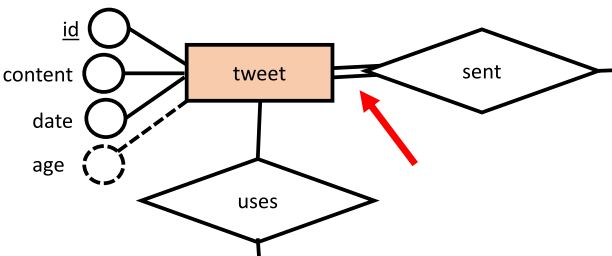
\includegraphics[scale=0.4]{Ex7.JPG}
\end{figure}

%%%%%%%%%%%%%%%%%%%%%%%%%%%%%%%%%%%%%%%%%%%%%%%%%%%%%%%%%%%%%%%%%%%%%%%%%%%%%%%%%%%%%%%%%%%%%%%%%%%%%%%%%%
\subsection{Self relations}

\begin{itemize}
    \item Label the two connecting lines to show \textbf{roles}
    \begin{figure} [h!]
        \centering
        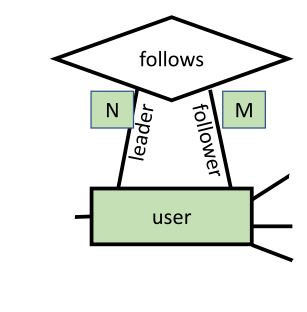
\includegraphics[scale=0.5]{Ex10.JPG}
    \end{figure}

    \item Cardinality constraints still apply
\end{itemize}

%%%%%%%%%%%%%%%%%%%%%%%%%%%%%%%%%%%%%%%%%%%%%%%%%%%%%%%%%%%%%%%%%%%%%%%%%%%%%%%%%%%%%%%%%%%%%%%%%%%%%%%%%%
\subsection{Relations with attributes}

\begin{itemize}
    \item Example: User can like a tweet with emojis
    \begin{figure} [h!]
        \centering
        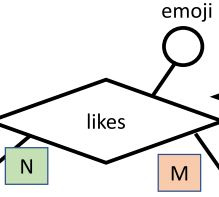
\includegraphics[scale=0.5]{Ex12.JPG}
    \end{figure}
\end{itemize}

\pagebreak

%%%%%%%%%%%%%%%%%%%%%%%%%%%%%%%%%%%%%%%%%%%%%%%%%%%%%%%%%%%%%%%%%%%%%%%%%%%%%%%%%%%%%%%%%%%%%%%%%%%%%%%%%%
\subsection{Three-way relationships}

\begin{itemize}
    \item Some relationships have more than two entity sets
    \item Example: User can \textit{watch} for new retweets
\end{itemize}
\begin{figure} [h!]
    \centering
    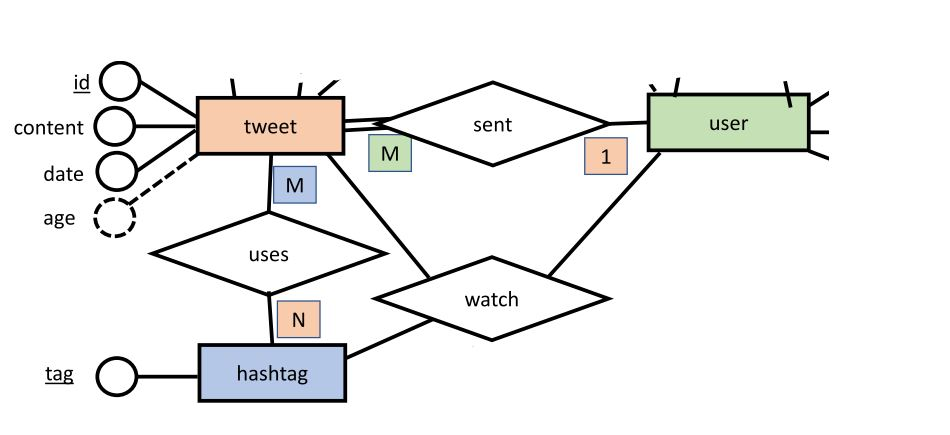
\includegraphics[scale=0.4]{Ex13.JPG}
\end{figure}

%%%%%%%%%%%%%%%%%%%%%%%%%%%%%%%%%%%%%%%%%%%%%%%%%%%%%%%%%%%%%%%%%%%%%%%%%%%%%%%%%%%%%%%%%%%%%%%%%%%%%%%%%%
\section{\textbf{ERM and Relations}}
%%%%%%%%%%%%%%%%%%%%%%%%%%%%%%%%%%%%%%%%%%%%%%%%%%%%%%%%%%%%%%%%%%%%%%%%%%%%%%%%%%%%%%%%%%%%%%%%%%%%%%%%%%

\begin{itemize}
    \item Entities can be mapped into relations i.e. ERM
    \item ERM captures important aspects of the world
    \item With an ERM, work can be done on data e.g. SQL
\end{itemize}

%%%%%%%%%%%%%%%%%%%%%%%%%%%%%%%%%%%%%%%%%%%%%%%%%%%%%%%%%%%%%%%%%%%%%%%%%%%%%%%%%%%%%%%%%%%%%%%%%%%%%%%%%%
\subsection{Relations}

\begin{figure} [h!]
    \centering
    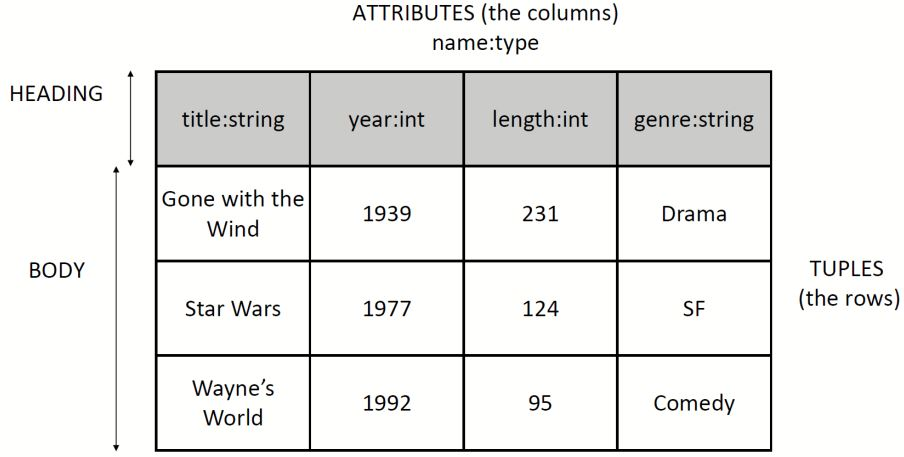
\includegraphics[scale=0.45]{Ex14.JPG}
\end{figure}

\begin{itemize}
    \item Relation composition:
    \begin{itemize}
        \item Relation Name
        
        \item Heading:
        \begin{itemize}
            \item Attributes:
            \begin{itemize}
                \item Name 
                \item Type
            \end{itemize}
        \end{itemize}
    
        \item Body:
        \begin{itemize}
            \item Tuples 
            \begin{itemize}
                \item Attribute value i.e. name and value
            \end{itemize}
        \end{itemize}
    \end{itemize}

    \item \textbf{Database}: Collection of relations
    \item \textbf{Relation Schema}: Relation name + Header
    \begin{itemize}
        \item \textit{movies(title:string, year:int, length:int, genre:string)}
    \end{itemize}
    \item \textbf{Database Schema}: Collection of relation schema
\end{itemize}

\pagebreak

%%%%%%%%%%%%%%%%%%%%%%%%%%%%%%%%%%%%%%%%%%%%%%%%%%%%%%%%%%%%%%%%%%%%%%%%%%%%%%%%%%%%%%%%%%%%%%%%%%%%%%%%%%
\subsection{ER diagrams $\rightarrow$ Relations $\rightarrow$ SQL}

\begin{itemize}
    \item Turning ER diagrams into concrete relations:
    \begin{itemize}
        \item ER attributes $\rightarrow$ Relation attributes 
        \item ER entity $\rightarrow$ Relations 
        \item ER relationship sets $\rightarrow$ Relations or may disappear 
    \end{itemize}

    \item Relations are then turned into SQL
\end{itemize}

%%%%%%%%%%%%%%%%%%%%%%%%%%%%%%%%%%%%%%%%%%%%%%%%%%%%%%%%%%%%%%%%%%%%%%%%%%%%%%%%%%%%%%%%%%%%%%%%%%%%%%%%%%
\section{\textbf{Structure Query Language (SQL) introduction}}
%%%%%%%%%%%%%%%%%%%%%%%%%%%%%%%%%%%%%%%%%%%%%%%%%%%%%%%%%%%%%%%%%%%%%%%%%%%%%%%%%%%%%%%%%%%%%%%%%%%%%%%%%%

\begin{itemize}
    \item Domain specific language
    \item Defines, query and updates data
    \item Mostly portable and often performance tuning required
    \item Composed of \textbf{tokens}:
    \begin{itemize}
        \item \textbf{Keywords}: CREATE, TABLE, SELECT \dots etc
        \item \textbf{Ordinary identifier}: \textit{x}, \textit{y}, \textit{movies}
        \item \textbf{Numbers}:3, 4.1, 1e-9
        \item \textbf{Delimited identifiers}: "Peter, Mary"
    \end{itemize}
    \item  SQL are case-sensitive
\end{itemize}

%%%%%%%%%%%%%%%%%%%%%%%%%%%%%%%%%%%%%%%%%%%%%%%%%%%%%%%%%%%%%%%%%%%%%%%%%%%%%%%%%%%%%%%%%%%%%%%%%%%%%%%%%%
\subsection{Creating a table}

\begin{verbatim}
CREATE TABLE movies (
    title varchar(100),
    year int,
    length int,
    genre char(16)
);
\end{verbatim}
\begin{figure} [h!]
    \centering
    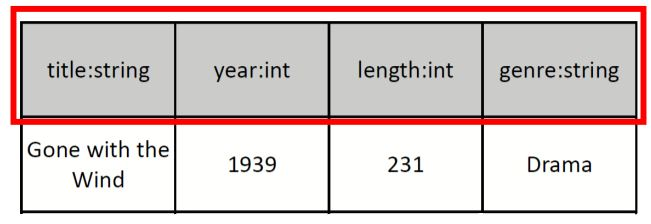
\includegraphics[scale=0.5]{Ex15.JPG}
\end{figure}

%%%%%%%%%%%%%%%%%%%%%%%%%%%%%%%%%%%%%%%%%%%%%%%%%%%%%%%%%%%%%%%%%%%%%%%%%%%%%%%%%%%%%%%%%%%%%%%%%%%%%%%%%%
\subsection{Inserting data into a table}

\begin{verbatim}
INSERT INTO movies
    VALUES (
    "Gone with the Wind”,
    1939,
    231,
    "Drama”
);
\end{verbatim}
\begin{figure} [h!]
    \centering
    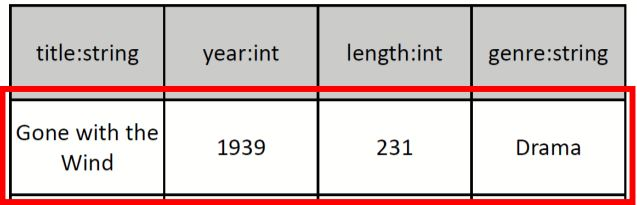
\includegraphics[scale=0.5]{Ex16.JPG}
\end{figure}

\pagebreak
%%%%%%%%%%%%%%%%%%%%%%%%%%%%%%%%%%%%%%%%%%%%%%%%%%%%%%%%%%%%%%%%%%%%%%%%%%%%%%%%%%%%%%%%%%%%%%%%%%%%%%%%%%
\subsection{Extracting data from table}

\begin{verbatim}
SELECT * from movies;
sqlite> select * from movies;

Gone with the Wind|1939|231|Drama
Star Wars|1977|124|SF
Wayne's World|1992|95|Comedy
\end{verbatim}
\begin{figure} [h!]
    \centering
    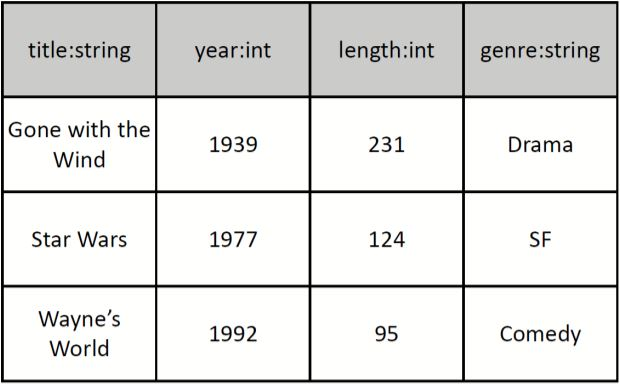
\includegraphics[scale=0.5]{Ex17.JPG}
\end{figure}

%%%%%%%%%%%%%%%%%%%%%%%%%%%%%%%%%%%%%%%%%%%%%%%%%%%%%%%%%%%%%%%%%%%%%%%%%%%%%%%%%%%%%%%%%%%%%%%%%%%%%%%%%%
\subsection{Extracting data from a table with filter}

\begin{verbatim}
SELECT * from movies WHERE year = 1977;

Star Wars|1977|124|SF
\end{verbatim}

%%%%%%%%%%%%%%%%%%%%%%%%%%%%%%%%%%%%%%%%%%%%%%%%%%%%%%%%%%%%%%%%%%%%%%%%%%%%%%%%%%%%%%%%%%%%%%%%%%%%%%%%%%
\section{\textbf{Mapping ERM to Relations}}
%%%%%%%%%%%%%%%%%%%%%%%%%%%%%%%%%%%%%%%%%%%%%%%%%%%%%%%%%%%%%%%%%%%%%%%%%%%%%%%%%%%%%%%%%%%%%%%%%%%%%%%%%%
\subsection{Entities and attributes}

\begin{itemize}
    \item Simple attributes: 
    \begin{itemize}
        \item Entity maps to relation with same attributes 
        \item Each entity in set becomes a row in relation 
        \item Entity primary key is relation primary key 
    \end{itemize}
\end{itemize}
\begin{figure} [h!]
    \centering
    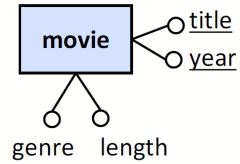
\includegraphics[scale=0.5]{Ex18.JPG}
\end{figure}
\begin{figure} [h!]
    \centering
    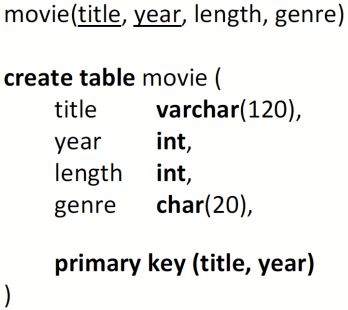
\includegraphics[scale=0.5]{Ex19.JPG}
\end{figure}

\pagebreak

\begin{itemize}
    \item Composite attributes:
    \begin{itemize}
        \item Composite attributes become list of attributes
    \end{itemize}
\end{itemize}
\begin{figure} [h!]
    \centering
    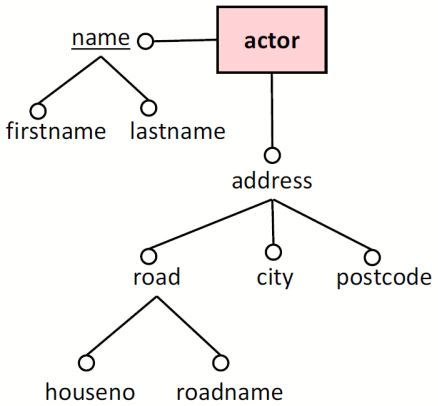
\includegraphics[scale=0.5]{Ex20.JPG}
\end{figure}
\begin{figure} [h!]
    \centering
    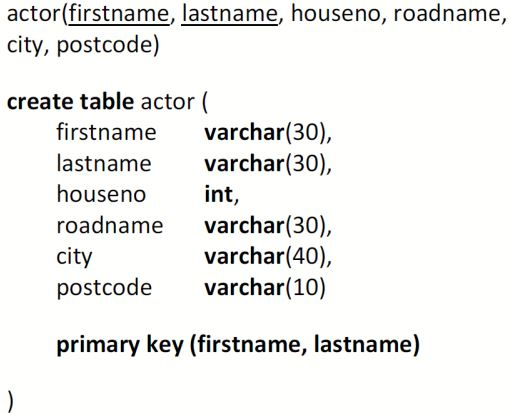
\includegraphics[scale=0.5]{Ex21.JPG}
\end{figure}

\begin{itemize}
    \item Multi-valued attributes:
    \begin{itemize}
        \item Attributes become own relation
        \item Relation linked to original set with \textbf{foreign key}
    \end{itemize}
\end{itemize}
\begin{figure} [h!]
    \centering
    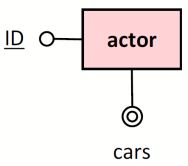
\includegraphics[scale=0.5]{Ex22.JPG}
\end{figure}
\begin{figure} [h!]
    \centering
    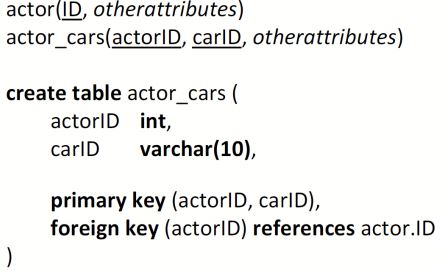
\includegraphics[scale=0.5]{Ex23.JPG}
\end{figure}

\begin{itemize}
    \item Derived attributes:
    \begin{itemize}
        \item Not directly supported
        \item Can be defined and used \textbf{within queries}
    \end{itemize}
\end{itemize}

\pagebreak
%%%%%%%%%%%%%%%%%%%%%%%%%%%%%%%%%%%%%%%%%%%%%%%%%%%%%%%%%%%%%%%%%%%%%%%%%%%%%%%%%%%%%%%%%%%%%%%%%%%%%%%%%%
\subsection{Relationship sets}

\begin{itemize}
    \item Many-to-many relationship:
    \begin{itemize}
        \item Relation with two foreign keys 
        \item Entity primary key is relation primary key 
    \end{itemize}
\end{itemize}
\begin{figure} [h!]
    \centering
    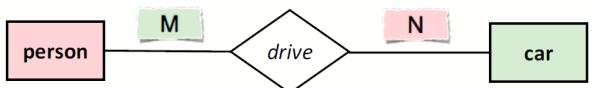
\includegraphics[scale=0.5]{Ex24.JPG}
\end{figure}
\begin{figure} [h!]
    \centering
    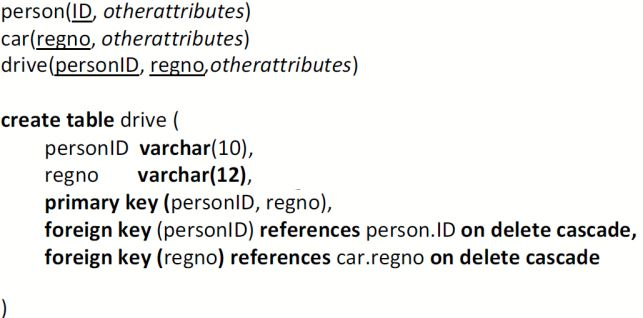
\includegraphics[scale=0.5]{Ex25.JPG}
\end{figure}

\begin{itemize}
    \item One-to-many relationship:
    \begin{itemize}
        \item Primary key of one as foreign key in another
    \end{itemize}
\end{itemize}
\begin{figure} [h!]
    \centering
    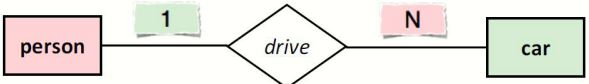
\includegraphics[scale=0.5]{Ex26.JPG}
\end{figure}
\begin{figure} [h!]
    \centering
    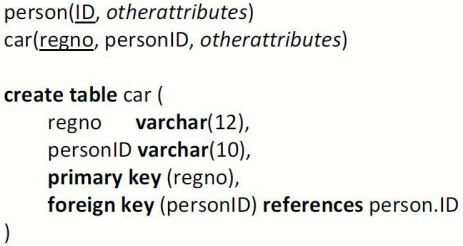
\includegraphics[scale=0.5]{Ex27.JPG}
\end{figure}

\begin{itemize}
    \item One-to-one relationship:
    \begin{itemize}
        \item Primary key of one as foreign key in another
    \end{itemize}
\end{itemize}
\begin{figure} [h!]
    \centering
    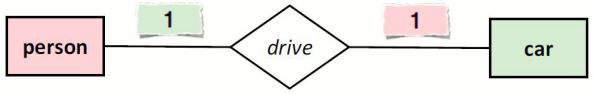
\includegraphics[scale=0.5]{Ex28.JPG}
\end{figure}
\begin{figure} [h!]
    \centering
    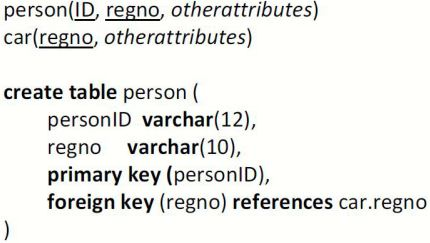
\includegraphics[scale=0.5]{Ex29.JPG}
\end{figure}

\pagebreak

\begin{itemize}
    \item Multi-way relationship:
    \begin{itemize}
        \item Form relation with foreign keys to entity sets
        \item Entity foreign keys form relation primary key
    \end{itemize}
\end{itemize}
\begin{figure} [h!]
    \centering
    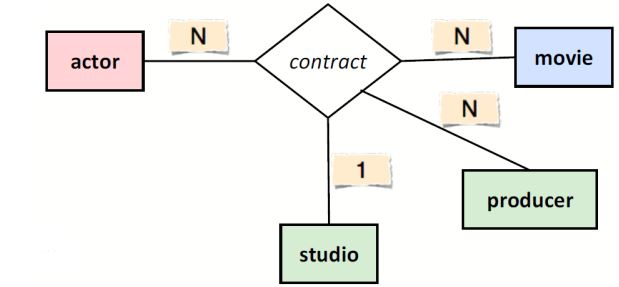
\includegraphics[scale=0.5]{Ex30.JPG}
\end{figure}
\begin{figure} [h!]
    \centering
    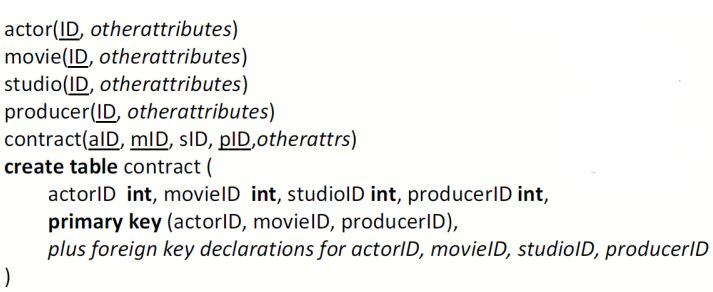
\includegraphics[scale=0.5]{Ex31.JPG}
\end{figure}

\begin{itemize}
    \item One-way relationship:
    \begin{itemize}
        \item Each role is foreign key on entity set
    \end{itemize}
\end{itemize}
\begin{figure} [h!]
    \centering
    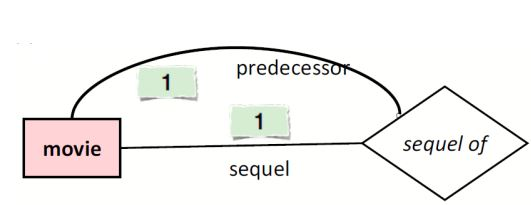
\includegraphics[scale=0.5]{Ex32.JPG}
\end{figure}
\begin{figure} [h!]
    \centering
    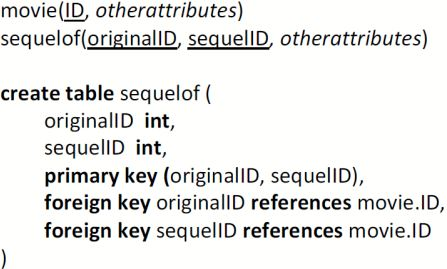
\includegraphics[scale=0.5]{Ex33.JPG}
\end{figure}


%%%%%%%%%%%%%%%%%%%%%%%%%%%%%%%%%%%%%%%%%%%%%%%%%%%%%%%%%%%%%%%%%%%%%%%%%%%%%%%%%%%%%%%%%%%%%%%%%%%%%%%%%%
\section{\textbf{Networks intro}}
%%%%%%%%%%%%%%%%%%%%%%%%%%%%%%%%%%%%%%%%%%%%%%%%%%%%%%%%%%%%%%%%%%%%%%%%%%%%%%%%%%%%%%%%%%%%%%%%%%%%%%%%%%

\begin{itemize}
    \item \textbf{Information}: Transmissible signal to receiver 
    \item \textbf{Data}: Information in machine-encoded form
    \item \textbf{Network}: Graph of nodes and channels:
    \begin{itemize}
        \item \textbf{Channel}: Path over which signals flow 
        \item \textbf{Node}: Device within network sending/receiving data 
    \end{itemize}
    \item Network metrics:
    \begin{itemize}
        \item Bandwidth: Throughout of many bytes 
        \item Latency: Delivery time for one byte 
        \item Jitter: Variation in latency 
        \item Loss: Proportion of bytes lost 
    \end{itemize}
\end{itemize}

\pagebreak
%%%%%%%%%%%%%%%%%%%%%%%%%%%%%%%%%%%%%%%%%%%%%%%%%%%%%%%%%%%%%%%%%%%%%%%%%%%%%%%%%%%%%%%%%%%%%%%%%%%%%%%%%%
\section{\textbf{Types of networks}}

\begin{itemize}
    \item Network switching: How network is implemented
    \begin{itemize}
        \item Circuit switching 
        \item Packet switching
    \end{itemize}
    \item Network connection service: What network offers to users
    \begin{itemize}
        \item Connectionless 
        \item Connection orientated
    \end{itemize}
\end{itemize}

%%%%%%%%%%%%%%%%%%%%%%%%%%%%%%%%%%%%%%%%%%%%%%%%%%%%%%%%%%%%%%%%%%%%%%%%%%%%%%%%%%%%%%%%%%%%%%%%%%%%%%%%%%
\subsection{Network switching}

\begin{itemize}
    \item Circuit switching: 
    \begin{itemize}
        \item Circuit maintained for duration of use 
        \item Three stages:
        \begin{itemize}
            \item Circuit establishment i.e. route established 
            \item Data transfer 
            \item Circuit disconnection
        \end{itemize}
        \item Only overheads are set-up costs
        \item Constant costs per unit time even if not in use 
        \item If any link/switch breaks, entire circuit breaks 
    \end{itemize}

    \item Packet switching: 
    \begin{itemize}
        \item Data sent as small packets of bits 
        \item Each packet routed independently
        \begin{itemize}
            \item Each packet must contain routing information
        \end{itemize}
        \item Packets may arrive out of order or get lost 
        \item Cost charged for each packet sent through 
    \end{itemize}
\end{itemize}
\begin{figure} [h!]
    \centering
    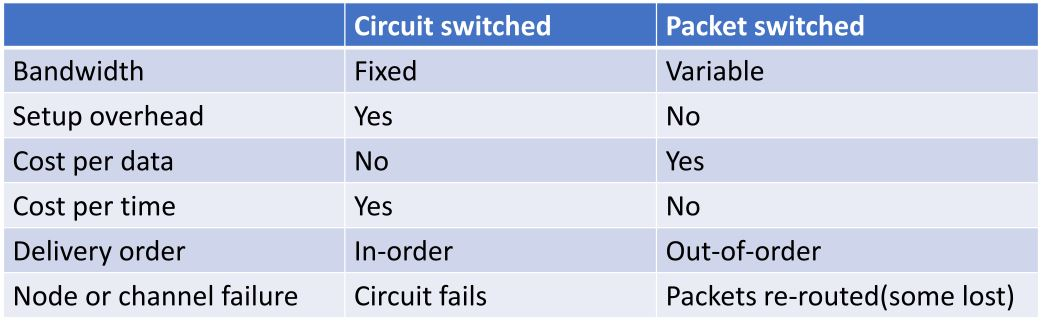
\includegraphics[scale=0.4]{Ex34.JPG}
\end{figure}

%%%%%%%%%%%%%%%%%%%%%%%%%%%%%%%%%%%%%%%%%%%%%%%%%%%%%%%%%%%%%%%%%%%%%%%%%%%%%%%%%%%%%%%%%%%%%%%%%%%%%%%%%%
\subsection{Types of connection service}

\begin{itemize}
    \item Connectionless service:
    \begin{itemize}
        \item No route is maintained
        \item Data is transmitted as packets 
        \item Packets may be re-ordered 
        \item No setups initially
        \item Similar to Packet Switching
    \end{itemize}
    \item Connection-orientated service:
    \begin{itemize}
        \item Route is maintained 
        \item Data transmitted as bytes along connection 
        \item Data arrives in the same order it was sent 
        \item Route established before data can be sent 
        \item Similar to Circuit Switching 
    \end{itemize}
\end{itemize}

\pagebreak
%%%%%%%%%%%%%%%%%%%%%%%%%%%%%%%%%%%%%%%%%%%%%%%%%%%%%%%%%%%%%%%%%%%%%%%%%%%%%%%%%%%%%%%%%%%%%%%%%%%%%%%%%%
\subsection{Virtual Circuit Switching}

\begin{itemize}
    \item Packeted-switching and Connection-orientated preferred
    \begin{itemize}
        \item Packet-switching: Robust routing, efficient sharing
        \item Connection-orientated: Reliable and in-order sending 
    \end{itemize}
    \item Virtual circuit provide connection using packets 
    \begin{itemize}
        \item Virtual circuit setup over packet-switched network
        \item Each node remembers virtual route  
        \item Data sent as packets along virtual connection 
        \item Packet are routed on established virtual route
    \end{itemize}
\end{itemize}

%%%%%%%%%%%%%%%%%%%%%%%%%%%%%%%%%%%%%%%%%%%%%%%%%%%%%%%%%%%%%%%%%%%%%%%%%%%%%%%%%%%%%%%%%%%%%%%%%%%%%%%%%%
\subsection{Quality of Service}

\begin{itemize}
    \item \textbf{Quality of Service} (QoS) guarantees: 
    \begin{itemize}
        \item Bandwidth: Minimum bandwidth along route  
        \item Latency: Maximum latency along route 
    \end{itemize}

    \item Circuit-switched: Worst channel in route 
    \begin{itemize}
        \item Determined when route is established
    \end{itemize}
    \item Packet-switched: QoS very difficult to guarantee
    \begin{itemize}
        \item Bandwidth varies according to demand 
        \item Latency varies according to channel congestion
    \end{itemize}
    \item Virtual circuit: QoS with \textbf{partial resource allocation}
\end{itemize}




%%%%%%%%%%%%%%%%%%%%%%%%%%%%%%%%%%%%%%%%%%%%%%%%%%%%%%%%%%%%%%%%%%%%%%%%%%%%%%%%%%%%%%%%%%%%%%%%%%%%%%%%%%
\end{document}
